\documentclass[main.tex]{subfiles}

\begin{document}

\subsection{Primo esercizio}

 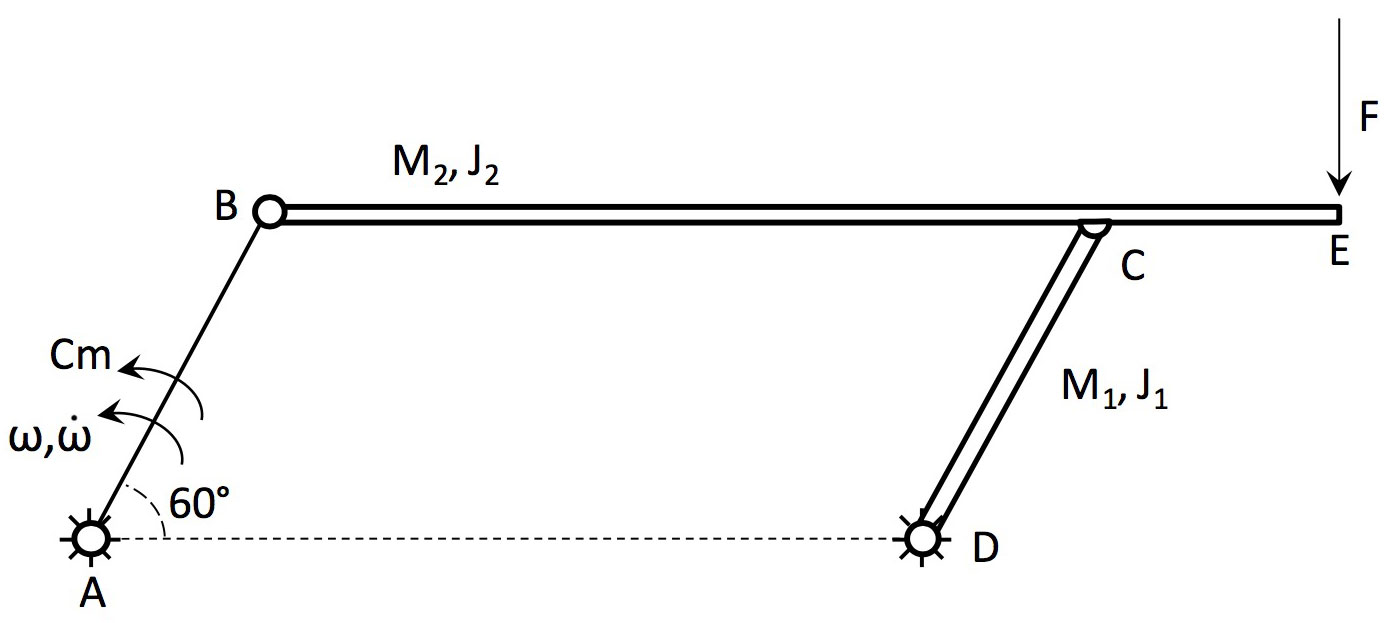
\includegraphics[width=\textwidth]{2015-2906-1.jpg}

\begin{alignat*}{5}
  J_2 = 1\,Kg\,m^2 \quad
  M_2 = 20\,Kg \quad
  J1 = 2\,Kg\,m^2\quad
  M_1 = 30\,Kg\quad
  BE = 1\,m\quad
\end{alignat*}
\begin{alignat*}{5}
  AB = CD = 0.5\,m\quad
  AD=BC=0.8\,m\quad
  F=500\,N\quad
  \omega = 5\,rad/s\quad
  \dot{\omega} = 0.5\,rad/s^2
\end{alignat*}


Il sistema rappresentato in figura è posto nel piano verticale.

L’asta AB, incernierata a terra in A, è collegata attraverso una cerniera in B all’asta BE che a sua volta è collegata attraverso una cerniera in C all’asta CD. Quest’ultima asta è incernierata a terra in D.

Si consideri trascurabile la massa dell’asta AB, mentre l’asta omogenea CD ha massa $M_1$ e momento d’inerzia baricentrico $J_1$ e l’asta omogenea BE ha massa $M_2$ e momento d’inerzia baricentrico $J_2$. Sull’asta AB, che si muove con velocit\'a angolare $\omega$ e accelerazione angolare $\dot{\omega}$ note, agisce la coppia $C_m$ incognita, mentre sul punto E è applicata in direzione verticale una forta $\vec{F}$ nota.
\\

Nota la geometria, si chiede di calcolare per la condizione di moto assegnata:
\begin{enumerate}
  \item la velocità e l'accelerazione del punto E.
  \item La coppia $C_m$ necessaria per garantire la condizione di moto assegnata.
\end{enumerate}

\pagebreak

\subsection{Soluzione primo esercizio}
\paragraph{Osservazioni importanti}
\begin{itemize}
  \item È \textbf{necessario} in questi esercizi intuire come il sistema si possa muovere.
  \item Nessuna asta cambia lunghezza (Questo può capitare in alcune condizioni, per esempio nel caso di \textit{glifo oscillante} o di \textit{compressore idraulico}).
  \item Gli unici oggetti con massa son l'asta BE e l'asta CD.
    \item Il sistema è posto sul piano verticale, quindi gli oggetti dotati di massa subiscono un'accelerazione verso il basso $g$ e ovviamente una forza peso $F_g$ che viene posta nel centro di massa.
  \item Nella struttura, le due aste inferiori agiscono come un \textit{doppio pendolo}, ognuna ha le caratteristiche di una \textit{biella} (o \textit{pendolo semplice}). L'asta superiore, di conseguenza, sarà sempre parallela al suolo e non avrà mai moto rotatorio ma solo traslatorio.
  \item L'asta BE è un corpo rigido in moto unicamente traslatorio. la velocità e l'accelerazione dovranno essere quindi uguale in qualsiasi punto (in particolare, $v_B = v_E$ e $a_B = a_E = a_{t_B} + a_{n_B}$).
  \item Il punto B può essere considerabile un punto posto su una circonferenza di raggio AB, con conseguenti leggi per \textbf{velocità} ($v_B = \omega r$), \textbf{accelerazione normale} ($a_{n_B} = \frac{v_B^2}{r}$) ed \textbf{accelerazione tangente} ($a_{t_B} = \dot{\omega}r$).
\end{itemize}

\clearpage

\paragraph{Primo punto}
Il calcolo di velocità ed accelerazione del punto E, in questo caso, risulta banale.

Riassumiamo i passaggi fondamentali per cui diventa immediato, già evidenziati più estensivamente nelle osservazioni sovrariportate:

\begin{enumerate}
  \item L'asta BE è un corpo rigido in moto esclusivamente traslatorio. Ogni suo punto, quindi, possiede la medesima velocità ed accelerazione.
  \item Il punto B è considerabile un punto posto su una circonferenza di raggio AB, per cui risultano applicabili le relative leggi del moto.
  \item Per rispettare la condizione di moto assegnata (come la coppia $C_m$ è direzionata) il versore $\vec{t}$ sarà orientato a $\frac{\pi}{2}+\frac{\pi}{3}$, mentre il versore $\vec{n}$ a $\frac{\pi}{2}+\frac{\pi}{3} + \frac{\pi}{2} = \pi + \frac{\pi}{3}$.
\end{enumerate}

\[
  v_B = AB\omega = 2.5\,m/s
\]

\[
  \vec{v}_B = 2.5\vec{t}\,m/s
\]

\[
  a_{t_B} = AB\dot{\omega} = 0.25\,m/s^2
\]

\[
  a_{n_B} = \frac{v_B^2}{AB} = \frac{AB^2\omega^2}{AB} = AB\omega^2 = 12.5\,m/s^2
\]

\[
  \vec{a}_B = 0.25\vec{t} + 12.5\vec{n}\,m/s^2
\]

\paragraph{Secondo punto}
Per calcolare la coppia $C_m$ proseguo col \textbf{bilancio di potenze} (figura \ref{bilancio_potenze}):

\subparagraph{Calcolo le potenze totali:}

\begin{align*}
  \sum W_i &= (\text{Coppie})\bullet(\text{Velocità angolari})\\
  &+ (\text{Forze peso})\bullet(\text{Velocità baricentriche}) \\
  &+ (\text{Forze})\bullet(\text{Velocità del punto di applicazione})
\end{align*}

\[
  \sum W_i = \vec{C}_m\bullet\vec{\omega} + \vec{F}_{g_{BE}}\bullet \vec{v}_{g_{BE}} + \vec{F}_{g_{CD}}\bullet \vec{v}_{g_{CD}} + \vec{F}\bullet \vec{v}_E
\]

La velocità baricentrica $v_{g_{BE}}$ è parte di un corpo rigido che non compie rotazioni, per cui è uguale a quella di qualsiasi altro punto. $v_{g_{BE}} = v_B$

La velocità baricentrica $v_{g_{CD}}$ è calcolabile tramite la formula usuale $v_{g_{CD}} = r\omega$, dove $r$ è la distanza dal centro di rotazione, in questo caso D, al baricentro dell'asta CD, per cui $r = \frac{CD}{2}$ e la velocità angolare $\omega$ coincide a quella di A, per cui $v_{g_{CD}} = \frac{CD}{2}\omega$.

\[
  \sum W_i = \vec{C}_m\bullet\vec{\omega} + M_2\vec{g}\bullet \vec{v}_B + M_1\vec{g}\bullet( \frac{CD}{2}\vec{\omega})  + \vec{F}\bullet v_B
\]

Risolvo il prodotto scalare, controllando direzione e verso dei vettori.

\begin{enumerate}
  \item La coppia $C_m$ e la velocità angolare $\omega$ sono date come orientate con stessa direzione e verso.
  \item La velocità $v_B$, per garantire il moto assegnato, è orientata verso l'alto con un angolo di $\frac{\pi}{2}+\frac{\pi}{3}$. Ovviamente la forza peso è orientata verso il basso, per cui l'angolo compreso tra i due vettori sarà pari a $\pi - \frac{\pi}{3}$.
  \item Discorso analogo per l'asta CD.
  \item Discorso analogo per l'asta BE
\end{enumerate}

\begin{align*}
  \sum W_i &= C_m\omega + M_2g v_{B}\cos(\pi - \frac{\pi}{3}) + M_1g( \frac{CD}{2}\omega)\cos(\pi - \frac{\pi}{3}) + F v_{B}\cos(\pi - \frac{\pi}{3}) \\
  &= C_m\omega - \frac{1}{2} M_2g (AB\omega) - \frac{1}{2}M_1g( \frac{CD}{2}\omega) - \frac{1}{2}F (AB\omega) \\
  &= C_m\omega - \frac{1}{4} M_2g \omega - \frac{1}{8}M_1g\omega - \frac{1}{4}F \omega \\
\end{align*}

\subparagraph{Calcolo l'energia cinetica totale:}
\begin{figure}[H]
\[
  E_{m_i} = \frac{1}{2}m_iv_{i_{baricentrica}}^2, \qquad E_{J_i} = \frac{1}{2}J_i\omega_{i}^2,
\]
\caption{Teorema dell'energia cinetica per le masse e per i momenti di inerzia}
\end{figure}

\begin{align*}
  E_c &= (\text{T. dell'en. cinetica per le masse})\\ &+ (\text{T. dell'en. cinetica per i momenti di inerzia})
\end{align*}

\[
  E_c = \frac{1}{2}M_2 v_{g_{BE}}^2 + \frac{1}{2}M_1 v_{g_{CD}}^2 + \frac{1}{2}J_1\omega_{CD}^2 +\frac{1}{2}J_2\omega_{BC}^2
\]

Alcune considerazioni sulle \textit{velocità angolari} presenti nell'equazione:

\begin{enumerate}
  \item Per le velocità vengono fatte le stesse considerazioni precedenti.
  \item $\omega_{BC}$ è l'accelerazione angolare dell'asta BC, ma questa non ruota affatto, il moto che compie è solamente traslatorio. Quindi $\omega_{BC} = 0$.
  \item $\omega_{CD}$ corrispende a $\omega_A$.
\end{enumerate}

\begin{align*}
  E_c &= \frac{1}{2}M_2 v_B^2 + \frac{1}{2}M_1 ( \frac{CD}{2}\omega)^2 + \frac{1}{2}J_1\omega^2 \\
      &= \frac{1}{2}M_2 (AB\omega)^2 + \frac{1}{2}M_1 ( \frac{CD}{2}\omega)^2 + \frac{1}{2}J_1\omega^2 \\
      &= \frac{M_2}{8} \omega^2 + \frac{M_1}{32}\omega^2 + \frac{1}{2}J_1\omega^2
\end{align*}

\subparagraph{Derivo l'energia cinetica totale e applico il bilancio delle potenze:}
\begin{figure}[H]
\[
  \sum_{i=0}^n W_i = \frac{dE_c}{dt}
\]
\caption{Bilancio delle potenze}
\label{bilancio_potenze}
\end{figure}

\begin{align*}
  \frac{dE_c}{dt} &= \frac{M_2}{4} \omega\dot{\omega} + \frac{M_1}{16}\omega\dot{\omega} + J_1\omega\dot{\omega}
\end{align*}

\begin{align*}
  C_m\omega - \frac{M_2}{4} g \omega - \frac{M_1}{8}g\omega - \frac{1}{4}F \omega &= \frac{M_2}{4} \omega \dot{\omega} + \frac{M_1}{16}\omega\dot{\omega} + J_1\omega\dot{\omega}\\
\end{align*}
Ora possiamo semplificare tutte le velocità angolari $\omega$ contemporaneamente:
\begin{align*}
  C_m - \frac{M_2}{4} g - \frac{M_1}{8}g - \frac{1}{4}F &= \frac{M_2}{4} \dot{\omega} + \frac{M_1}{16}\dot{\omega} + J_1\dot{\omega}\\
  C_m - 5 g - \frac{15}{4}g - 125 &= 5 \dot{\omega} + \frac{15}{8}\dot{\omega} + 2\dot{\omega}\\
\end{align*}
\begin{align*}
  C_m &= 5 \dot{\omega} + \frac{15}{8}\dot{\omega} + 2\dot{\omega} + \frac{35}{4}g + 125\\
  C_m &=  \dot{\omega}(5 + \frac{15}{8}+ 2) + \frac{35}{4}g + 125\\
  C_m &=  \frac{1}{2}(5 + \frac{15}{8}+ 2) + \frac{35}{4}g + 125\\
\end{align*}
Posto $g=9.81m/s^2$ risolvo:
\begin{align*}
  C_m &=  \frac{1}{2}(5 + \frac{15}{8}+ 2) + \frac{35}{4}9.81 + 125\\
      &= 215,275 Nm \\
      &\approx 215 Nm
\end{align*}
\clearpage

\end{document}